\def\year{2015}
%File: formatting-instruction.tex
\documentclass[letterpaper]{article}

% Required Packages
\usepackage{aaai}
\usepackage{times}
\usepackage{helvet}
\usepackage{courier}
\usepackage{graphicx}
\frenchspacing
\setlength{\pdfpagewidth}{8.5in}
\setlength{\pdfpageheight}{11in}

\graphicspath{{./image/}}

% Section numbers. 
\setcounter{secnumdepth}{2}  

\nocopyright
\begin{document}
% Title and author information
\title{Assignment 3 report - Group: YSoSirius \\ 02285 AI \& MAS}
\author{Bogdan Sorlea \\ s121075 \And Rasmus Kr{\o}yer J{\o}rgensen \\ s090487}
\maketitle
\begin{abstract}
This paper presents YSoSirius Group's solution to the 02285 - AI \& MAS 2015 competition. We will be describing the theoretical background for our solution, the methods and the implementation, discuss the results and reason about how to improve this solution. Our approach is based on several ideas which include goal decomposition, associating priorities to goals, pre-computing static metrics to aid with improving the heuristics function and conflict solving.
\end{abstract}

\section{Introduction}
In this paper we are presenting our solution to the 02285 - AI \& MAS 2015 competition. The aim of the competition is to find clever and efficient solutions to multi-agent problems in Artificial Intelligence.

The present competition presents the challenge of designing and tuning a system for solving multi-agent worlds (levels) in which various agents (represented by robots) have the ability to move with the aim of pushing or pulling various items ("boxes") in order to move them to their final position ("goal").

This problem has a lot of relevance in applications that require the automation of human-less deliveries of goods and the solutions can be applied to a plethora of situations, from warehousing solutions to hospital supply planning and other specialized delivery systems.

We have chosen a solution based on goal decomposition, pre-computing static data that aids in searching and conflict resolution. We have started with optimizing the solution for a single-agent scenario, in which we chose to prioritize goals based on how much a goal was blocked by others - to help with reducing conflicts, we pre-computed "distance map" metrics for each goal - to improve the heuristics function, especially since this was static data. 

Since this implementation was efficient enough, we decided to move onto solving the multi-agent levels as best as possible, although we had other ideas on how to improve searching. However, we are discussing these solutions in the \textit{Future Work} section. For the multi-agent levels we focused on efficiently doing conflict solving, the process around this being described in the \textit{Methods} chapter.

\section{Background}
The design of our client is based on several of the theories learned in this course. The main one is the the BDI architecture even though our client only partly implements the model. 

As the \textit{desires} we have all the goal cells that needs to be solved. As the \textit{intentions} we have the specific goal cell that an agent wants to solve. Below this is called a sub-goal. The \textit{beliefs} of the agents is a copy of a variable that holds the current state of the map with all agents and boxes. We use a blackboard achitecture, so the original \textit{currentState} varialbe is always available to all agents and it is updated each time an action is taken. There is little difference between the \textit{perceptions} and \textit{beliefs} of an agent in our solution.

Our client implements \textit{plan monitoring} and \textit{online replaning}. We initially considered using offline planning with plan merging, but the possible complexity of the solutions seemed to be cumbersome to work with. We have also implemented \textit{goal monitoring}. Even though a sub-goal is always assumed to be achievable, a plan to solve it might be dropped in favor or conflict resolution and replanning. A feature that our client does not have is \textit{online deliberation}, since we believed it would not be worth it in terms of computational ressources. 

\section{Related work}
Research needs to be done. This section could be moved.

\section{Method}
This section contains a detailed explanation of the algorithm our client uses. Each step will be explained in its own section. There will less focus on the theory behind this solution as this should be clear from the previous section.

\begin{figure}[!htb]
\centering
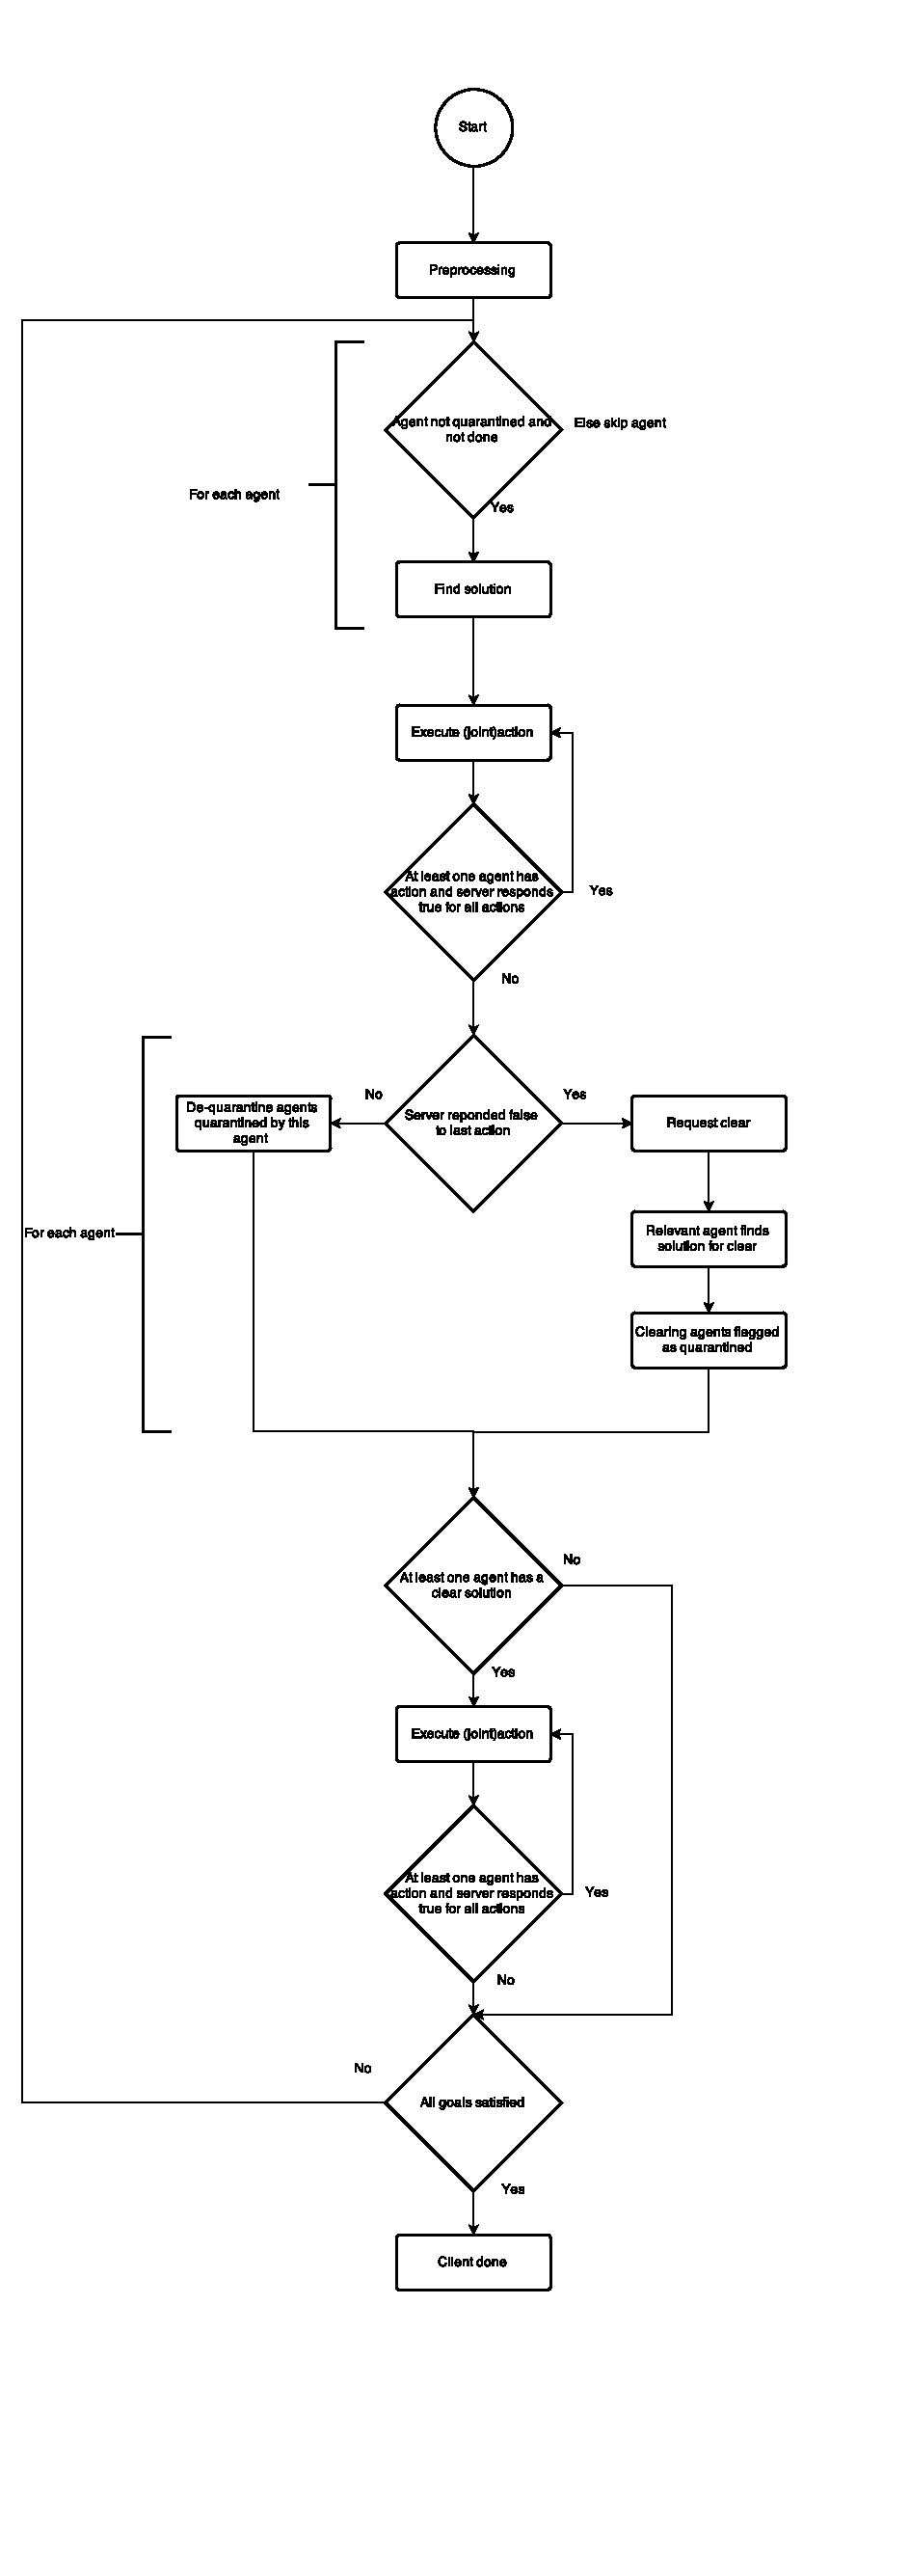
\includegraphics[scale=0.45]{ClientFlowchart.pdf}
\caption{Flowchart of the base client loop}
\label{fig:clientFlowchart}
\end{figure}

Figure \ref{fig:clientFlowchart} shows a visual reprensentation of the main client loop.

\subsection{Preprocessing}
The first step upon start-up is the pre-processing step. This step is not part of the core loop of the client and will only be executed once. In this part we first read the input to the server to create our perception of the map. After this we perform a simple form of goal decomposition. Each goal cell is treated as a independent goal that must be achieved. Then for each goal we calculate the goal priority. The priority is based on whether or not other goal cells block this goal cell - that is if by solving the other goals you will then block access to this goal. Once each goal cell has a priority we then calculate the exact distance from each cell to each goal cell. This will help us have a more efficient heuristic when we want to know the distance from the boxes to the goal cells.

\subsubsection{Distance map}

While incrementally developing the solution, we took the decision to simplify as much as possible, wherever it was possible. One such simplifications relied on pre-computing a distance map for each of the goal cells. The rationale behind it was that if we could obtain a solution that is not computationally intensive for computing the minimum distances from each cell to each goal cell, as the goal cells stay constant (a goal cannot be moved), then we would have a very precise metric to include in our heuristic function, which would ultimately make the solution more robust.

For computing this distance map we took an approach based on starting from the goal cell and, using the 4-vicinity, continuously add neighbors into a frontier list, that would be continuously processed until empty. The processing consists of always storing the minimum distance to a specific cell, which is based on the distance to its parent, incremented by one.

The usage of the frontier data structure and of the way the distance is computed can be considered to be structurally similar to how the best-first strategy algorithm work - which itself is an important part of the solution, in exploring the state space.

Specific measures were taken in order to increase the performance of the algorithm, most important one being a check based on which the iteration would just continue if a specific cell has been already processed (i.e. due to a different - and therefore possibly shorter - path from the goal to that specific cell).

The result of applying the aforementioned algorithm is a map of distances similar to the one in Figure \ref{fig:distmapb}, which corresponds for the level in Figure \ref{fig:distmaporig} and the goal denoted by \textit{b}.

\begin{figure}[!htb]
\centering
\begin{minipage}[b]{0.45\linewidth}
	\centering
	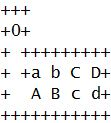
\includegraphics[scale=0.4]{distmap_orig.JPG}
	\caption{Original level}
	\label{fig:distmaporig}
\end{minipage}
\quad
\begin{minipage}[b]{0.45\linewidth}
	\centering
	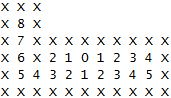
\includegraphics[scale=0.5]{distmap_b.JPG}
	\caption{Distances to \textit{b}}
	\label{fig:distmapb}
\end{minipage}
\end{figure}

It is noteworthy that the algorithm itself does not take into account situations where a level is split into two or more disjoint areas, where one area is not reachable from another and this might lead to exceptions in some levels. Therefore, this scenario can be improved by map initialization to an arbitrary flag that indicates that the cell has not been reached in any way from the goal.

\subsection{Find solution}
In relation to the BDI architecture this step involves updating the Beliefs, Desires and Intention of each agent. In this step each agent will first update their desire, which in our context is to find a new sub-goal (found from the goal decomposition mentioned above). If the agent does already have a goal and this is not yet achieved then no new goal is given. If the agent is not done and is not quarantined (explained later) then it is given an updated version of the map and the positions of agents and boxes. From this state the agent uses a graph search tree with a heuristic function to find a state that satisfies its goal. During this search process the agent assumes that the map stays unchanged, except for the changes made by the agent. The agent also cannot see obstacles in the form of boxes of another color or other agents, so it will plan as if they are not there (but these can still influence the heuristic function).

\subsubsection{Heuristic function}
The heuristic function we use is a relaxed, admissible heuristic function. It uses the A* as its basis which means that it will add a $g()$ function to all heuristics. The $g()$ functions return the number of steps to the initial state of the search tree. The $h()$ part of the heuristic function is found in the following way. It will find the box closest to the goal cell that the agent is trying to solve and then find the distance between the two, using the goal distance map we calculated during the pre-processing. It will then find the Manhattan distance between the agent and the box chosen and add that to the earlier distance found and this will be the foundation of the returned value. There are few other things that influence the heuristic:
\begin{itemize}
\item Moving a box that is not the box found earlier will add to the returned value
\item Moving a box or the agent into a cell the is occupied by another box or agent will add to the returned value.
\item Moving a box or the agent into a cell that is a solved goal cell will add greatly to the returned value.
\end{itemize}
Since the search function will chose the state whose heuristic function returns the lowest value, adding to the value returned effectively discourages the agent from choosing that state. \textit{Possibly explain why heuristic is admissible and relaxed}.

\subsection{Execute plan}
Once each agent has a plan that will solve its current subgoal, the plan will be executed. The loop that executes the plan will terminate if the server responds \textit{false} to any of the actions given - that is if the action an agent is trying to do is not possible. The client has a blackboard architecture and has a shared variable that holds the current state of the map. This variable is updated each time and agent has performed an action successfully. It is the same variable that an agent copies when it updates its beliefs in the previous stage. Once all agents have executed their plan the loop terminates, assuming it was not terminated prematurely because of a conflict.

\subsection{Conflict resolution}
When the loop mentioned above ends, a check is made for each agent to find out if its last action results in an error. If there was no error then all plans were executed successfully and this step is skipped. However, if an agent ended the loop with an error, then this agent will request the cells that it is going to occupy in the next action of its plan to be cleared. It will send this request to all other agents, and if either the agent itself occupies one of the cells to be cleared, or if the agent has the same color as a box that occupies a cell to be cleared, then this agent will search for a plan to clear these cells.

Because the next action will always only occupy one new cell, it will also always only need one agent to help do the clear. In an earlier iteration of the system the agent would request all cells that will at one time get occupied in its plan to be cleared, and the fact that it sends the clearing request to all agents is a remnant of this system. This is discussed furter in the discussion section.

The heuristic function used to find a plan for clearing cells is different than the one used to find a plan for achieving sub-goals. It is also an A* heuristic, but here we calculate the aggregated distance to the cells that needs to be cleared, as well as adding a big reward in terms of heuristic value when a cell is cleared. This function also tries to encourage the agent to go around obstacles that it cannot move.

Once all agents that needs to clear have a plan, the plan will be executed in the same manner as descibed earlier. Again the loop is terminated when all agents have finished their plans, or when an agents action results in an error. This means that an agent resolving a conflict cannot get help from other agents in case it is blocked. This approach has some issues which we will discuss in the discussion section.

If an agent has to move a box that is solving a goal cell, then the goal cell is added again to the list of sub-goals but with a lower priority.

When an agent finds a clearing solution it will also be flagged as quarantined, which means it will not search for a solution for its sub-goal in the next iteration of the loop. This is in order to ensure that the agent will not intervene with the path of the agent it has just cleard for. When the \textit{Execute Plan} phase is done, all agents are unflagged as quarantined, if the agent that quarantined them successfully finished its plan. 


\section{Results}
Discuss our results.

\section{Discussion}
... Moved this from Introduction, where I initially started writing it:

where, due to the pre-computation of what we call "distance map" the solutions to these levels were quite optimal in terms of time. It is noteworthy that we also tried to prioritize the solving of the goals based on situations where one goal might be blocked by another (or several) and, although efficient for most levels, this has proven catastrophic for levels like "SAboxesOfHanoi.lvl". Nonetheless, we decided to continue with this solution, both due to time and code complexity limitations.

\section{Future work}
For future work we consider some of the ideas we had during the implementation, but for various reasons we decided not to include them. We will be describing the ideas, the benefits and well as the disadvantages and other notable details.

\subsection{Reducing the state space}
One idea we considered at an early stage in the project was to try and reduce the state-space of each level, thus reducing the complexity of searching in this state-space. The abstract description on how to achieve this is by removing some of the cells in the level, for example by marking them (in a separate data structure than the one storing the original level) as being walls, such that the overall function of the level is not perturbed (i.e. all paths from agents to boxes and from boxes to goals are still valid after running the algorithm that reduces the state-space).

Applying such an algorithm will result in a level with more wall cells, therefore less cells that can be occupied by an object (box, agent or goal), resulting in a decreased complexity while searching, by reducing the base of the exponential function that defines this complexity (by the number of converted cells), therefore reducing the search's branching factor.

While this improves performance while searching, it has the disadvantage of making conflict resolution more cumbersome, unless special procedures are considered in this case. One such procedure can be conflict solving in the original state-space (in the original layout of the level), while all other search taking place in the reduced state-space. Another consequence of such an implementation is an increased probability of conflicts, as the chances of bottlenecks being formed are higher.

This idea can be implemented based on an algorithm in Image Processing and Computer Vision called "dilation", a morphological step used in various algorithms, e.g. removing noise from an image. The details of this algorithm can be consulted in [make proper reference: http://users.utcluj.ro/~igiosan/Resources/PI/L7/PI-L7e.pdf], but in our case it translates to a simple routine: it would mark a non-wall cell as wall cell if at least one of the cell's neighbors in its 4-vicinity is a wall cell. The union of this set of newly marked wall cells and the walls in the original level (or walls in the previous iteration, if applied iteratively) will form the final walls in the level.

This is an efficient implementation, not computationally complex, but however, it has some disadvantages we are still thinking how to best overcome. The disadvantages are given by the complex nature of the reasoning that will assure that at each dilation iteration we are not isolating any of the cells of interest, i.e. boxes, goals or agents. While we have thought about this problem and we have some ideas on how to overcome it, we would first have to experiment with some strategies before we would be able to strongly claim any solution. Therefore, we are just raising awareness on the issue but not offering a concrete solution at this time.

On a related topic, another challenge to iterative dilation is reasoning about when to stop dilating the walls of the level. This is also something to experiment with and therefore no solution would be provided here.

An example of this level transformation works can be seen in Figure \ref{fig:level_before_dilation} and Figure \ref{fig:level_after_dilation}, where in Figure \ref{fig:level_before_dilation} we see the original walls of the level and in Figure \ref{fig:level_after_dilation} we see the final walls after the dilation (run for 1 iteration, based on the 4-vicinity kernel). Note that in Figure \ref{fig:level_after_dilation} we have ignored the walls that would be computed outside the bounds of the original level, as are they deemed irrelevant.

\begin{figure}[!htb]
\centering
\begin{minipage}[b]{0.45\linewidth}
	\centering
	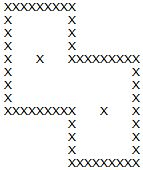
\includegraphics[scale=0.4]{level_before_dilation.JPG}
	\caption{Walls before dilation}
	\label{fig:level_before_dilation}
\end{minipage}
\quad
\begin{minipage}[b]{0.45\linewidth}
	\centering
	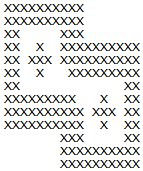
\includegraphics[scale=0.5]{level_after_dilation.JPG}
	\caption{Wall after dilation (1 iteration)}
	\label{fig:level_after_dilation}
\end{minipage}
\end{figure}

We have decided not to proceed with experimenting and implementing this solution at an early stage in the project. There are two main reasons behind this decision: we saw this as possibly complicated in terms of the algorithm, provided that all functional safety measures are to be taken in regards to the level and we found other ideas as more efficient (e.g. computing a distance map for each of the goals) and therefore considered that such a solution might not bring a huge benefit. However, it is an interesting idea that is worth an investigation, as the complexity of the resulting algorithm would most likely be fairly small, \textit{O(m*n)}, where \textit{m} and \textit{n} are the dimensions of the original level.

\subsection{Improving the informed search}
We also considered various strategies for improving the way the heuristics function is computed (by incorporating various metrics or flags into the heuristics function). One such strategy is to be applied only for the sub-goal of an agent reaching a box, as the sub-goal of the agent and box reaching the goal is accurately and easily solvable by the distance map computed for each goal.

As the heuristic function relies on Manhattan-distance-like metric, this is not in any way helpful if any direct path between the agent (source) and box (destination) is blocked by walls - as all the actual paths will be searched last, i.e. after the direct paths are unsuccessfully searched.

Therefore, to improve situations like these we could either do ad-hoc quick searches for blocked paths between a source and a destination coordinate, or such computations could be done globally, for all the walls within the level, as a pre-processing step. However, this second approach might be too cumbersome to compute and therefore inefficient, especially since it would compute such a flag ("is there at least one direct path between source and destination?") for each (source, destination) pair, even if most of them would not be ever used.

However, computing such a flag on-demand, while storing the relevant information in a constructive way, such that successive computations can rely - at least in part - on previous computations' data, might be efficient enough as to stand as a mid-point in terms of computation between levels with a lot of direct-path sub-goals (in which the search is done effectively) and levels with few to none such direct-paths (in which the search is quite inefficient and therefore time and resource consuming).

The algorithm is to be implemented in such a way as to start from one end (e.g. source) and move towards the destination, continuously checking if each neighbor of a specific cell in the two valid directions (directions that get the position closer to the destination, on either the horizontal or vertical lines) is still reachable. If unreachable, it is due to the neighbor being a wall and therefore any further computation with that neighboring cell is stopped - by not adding that neighbor to a "frontier" list of cells that are still valid. By doing this search as BFS and running until the frontier list is empty, we can obtain an answer of whether the destination is directly-reachable from source. At the end of the algorithm, some post-processing should be done, as to globally save the information on which cells could not be reached (and from which cells) and at each iteration relevant information on the progress should be globally saved, as it might be used by any subsequent checks. This reflects the fact that a check from source to destination can be decomposed in many adjacent checks between two cells lying in the space between the source and destination, and any of the computed flags in a specific computation might be used in a subsequent computation to reduce the complexity. Therefore the algorithm can be viewed and should be implemented as a \textit{Divide et Impera} problem, where the results of sub-problems are cached to reduce complexity of subsequent runs.

Based on this flag a decision to start searching in the opposite direction than the direct moves can be taken, whenever this flag is not favoring searching by direct Manhattan procedure. In terms of heuristics, this is accomplished by introducing a penalty to the direct Manhattan metric whenever this check fails.

\section{Bibliography}
Your bibliography should be formatted using \texttt{aaai.bst} as this document. Citations are included like so~\cite{book2015}. Multiple citations appear like this~\cite{conf,article}. All references to be cited should be included in BibTeX format in the file \texttt{bibliography.bib}.\footnote{Almost anything ever published can be found in BibTeX format via Google Scholar, but if using this method, you need to check the BibTeX entry for sanity before including it in the \texttt{bibliography.bib} file.}



% References and end of paper
\bibliographystyle{aaai}
\bibliography{bibliography}

Remove this if not needed anymore (render of flowchart as jpg)

\begin{figure}[!htb]
\centering
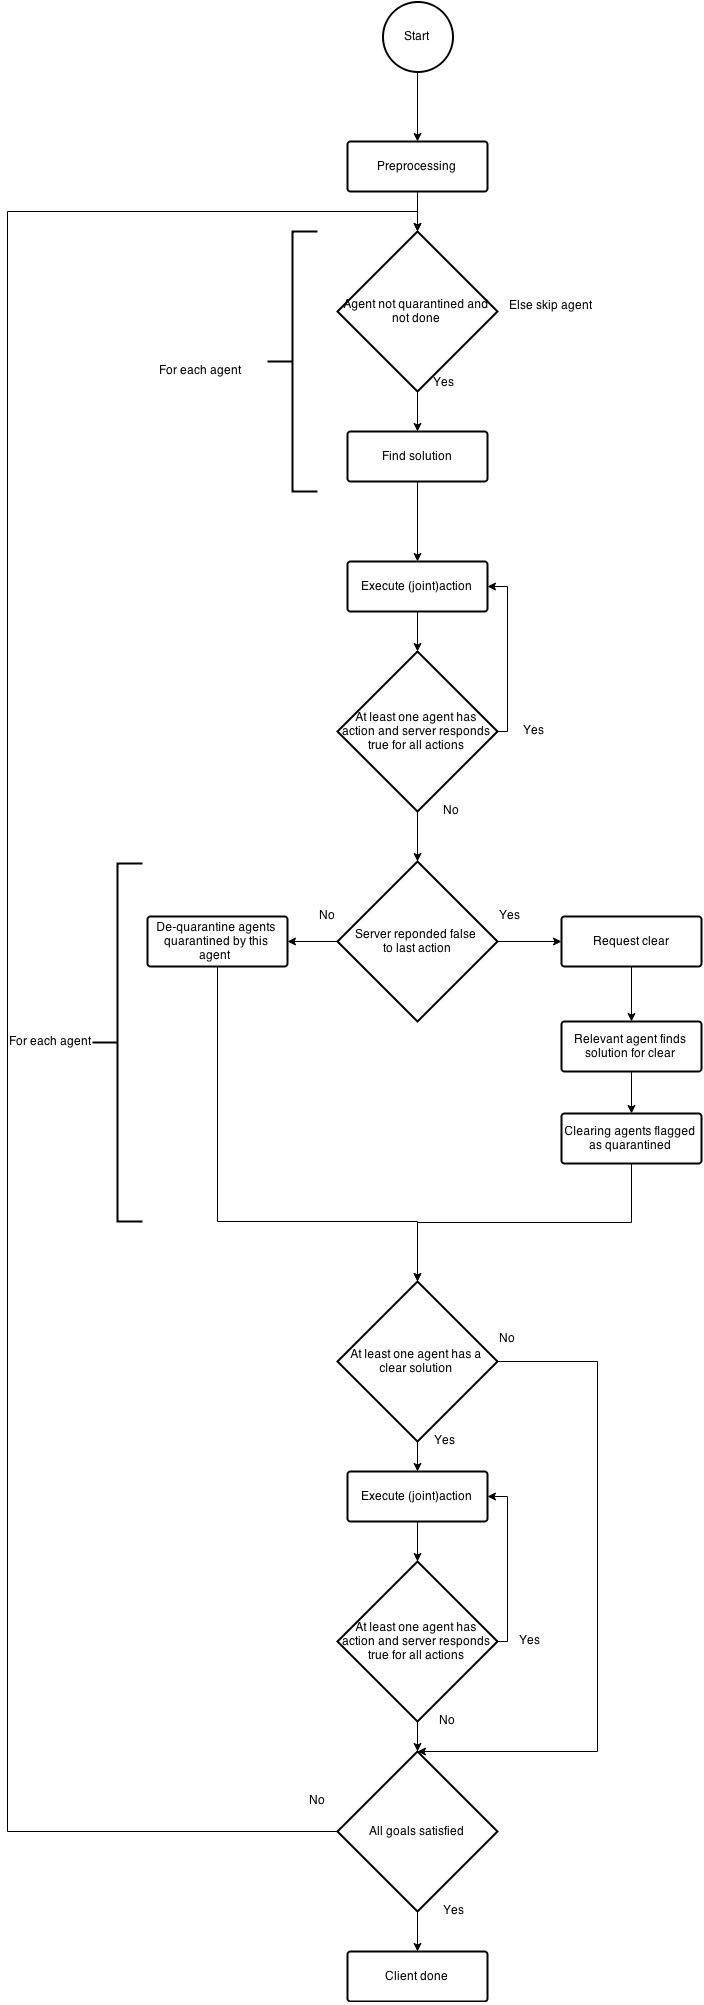
\includegraphics[width=\linewidth]{clientflowchart.jpg}
\caption{Flowchart of the base client loop}
\label{fig:clientflowchart}
\end{figure}

\end{document}
